\documentclass{article}

\title{If composers were hackers}
\subtitle{What programming language would J.S. Bach use?}
\date{2023-04-01}
\modified{2023-04-01}

\keyword{programming}
\keyword{personal}
\keyword{glasperlenspiel}

\begin{document}
\section{introduction}{Introduction}

Music is my first true love\sidenote{zero-love}{Computer games are my zeroeth true love.}.
The first time I got my hands on an old untuned guitar, I didn't want to put it down.
I found a summer job to buy my first instrument and pay for a teacher, and since then, music has been a constant source of joy in my life.
Picking a degree in computer science at a university over a musical college education was a hard choice for me.

I can't help but look at the world through my musical obsession.
There are many deep similarities between music and computing but we won't explore them in this article.
Instead, I will focus on a silly and subjective question: ``If my favorite composers decided to write some code, which language would they pick?''

\section{bach}{Johan Sebastian Bach}

\href{https://en.wikipedia.org/wiki/Johann_Sebastian_Bach}{Johan Sebastian Bach} is the most talented and prolific musician in history.

Bach would love the \href{https://en.wikipedia.org/wiki/APL_(programming_language)}{APL} programming language:

\begin{itemize}
  \item
    Like a well-written APL program, Bach's music is \em{dense}.
    He achieves immense expressive power with a few well-chosen constructs.
  \item
    In his lifetime, Bach was famous not for his compositions, but for his improvisation skills.
    APL is an excellent fit for live coding because of its interactivity and terseness.
  \item
    Motifs and keys bear deep symbolic and emotional meaning in Bach's music.
    A twisted motif might mean a crucifixion and a sequence of twelve beats might depict a clock striking midnight.
    APL assigns ingeniously-chosen symbols to all its primitives.
  \item
    Bach's productivity was phenomenal.
    For example, he was cranking at least one cantata (about 20 minutes of music) per week for church services on Sundays for over three years, writing over three hundred cantatas.
    And it wasn't even his primary duty.
    Tell me about your tight deadlines.
    The only programmer who can come close to this level of productivity must be an over-caffeinated APL wizard.
  \item
    The \href{https://en.wikipedia.org/wiki/Contents_of_the_Voyager_Golden_Record}{Voyager Golden Record} contains three compositions by Bach.
    If we wanted to prove to aliens that we know how to compute, APL would be the best choice for writing programs on golden surfaces.
\end{itemize}

\begin{figure}[grayscale-diagram]
  \marginnote{mn-repr-bach}{
    Representative Bach's music: \em{Wachet auf, ruft uns die Stimme}, a deeply moving and masterfully harmonized choral.
  }
  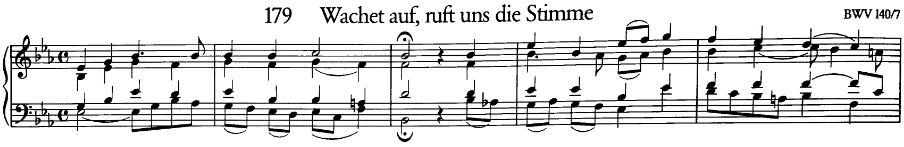
\includegraphics{/images/18-bach-snippet.png}
\end{figure}
\begin{figure}
  \marginnote{mn-apl-program}{
    An APL function computing \math{2\sup{n}} \href{https://en.wikipedia.org/wiki/Gray_code}{Gray codes} for the given number \math{n}.
    This code comes from \href{https://www.jsoftware.com/papers/50/}{A History of APL in 50 functions} by Roger K.W. Hui.
    \href{https://tryapl.org/?clear&q=%7B(0%E2%88%98%2C%20%E2%8D%AA%201%E2%88%98%2C%E2%88%98%E2%8A%96)%E2%8D%A3%E2%8D%B5%E2%8D%89%E2%8D%AA%E2%8D%AC%7D%C2%A8%202%203%204&run}{Try it yourself!}
  }
  \center{
    \begin{code}[apl]{(0∘, ⍪ 1∘,∘⊖)⍣⍵⍉⍪⍬}\end{code}
  }
\end{figure}

\subsection{bach-apl-resources}{Resources}

If you want to learn more about J.S. Bach:
\begin{itemize}
  \item
    Listen to the \href{https://www.thegreatcourses.com/courses/bach-and-the-high-baroque}{Bach and the High Baroque} course\sidenote{sn-audible-gc}{
      \href{https://audible.com}{Audible.com} offers subscribers all courses I mention in this article for free or at a meager price.
    } by professor \href{https://robertgreenbergmusic.com/}{Robert Greenberg}.
  \item
    Read \href{https://www.amazon.com/Johann-Sebastian-Bach-Musician-Paperback-ebook/dp/B002GKGBLE}{Johan Sebastian Bach: The Learned Musician} by Christoph Wolff.
\end{itemize}

If you want to learn more about APL:
\begin{itemize}
  \item
    Read \href{https://en.wikipedia.org/wiki/Kenneth_E._Iverson}{Ken Iverson's} ACM Turing Award lecture \href{https://dl.acm.org/doi/10.1145/358896.358899}{Notation as a Tool of Thought}.
    The \href{https://www.jsoftware.com/papers/}{jsoftware website} hosts this and many other papers on APL.
  \item
    Read \href{http://www.dyalog.com/mastering-dyalog-apl.htm}{Mastering Dyalog APL} book by Bernard Legrand and play with the \href{https://tutorial.dyalog.com/}{Dyalog APL Tutorial}.
  \item
    Listen to the \href{https://arraycast.com/}{ArrayCast} and \href{https://apl.show/}{APL.Show} podcasts.
  \item
    Watch the \href{https://youtu.be/DsZdfnlh_d0}{Depth-first search in APL} video for inspiration.
  \item
    Consider getting a physical copy of \href{https://www.amazon.com/APL-Interactive-Approach-Leonard-Gilman/dp/0471093041}{APL: An Interactive Approach} book by Leonard Gilman and Allen J. Rose.
    The content is pretty dated, but this book is one of the most engaging books on programming I've ever read.
\end{itemize}

\section{mozart}{Wolfgang Amadeus Mozart}

\href{https://en.wikipedia.org/wiki/Wolfgang_Amadeus_Mozart}{Mozart}'s musical genius was so bright and incomprehensible that mysteries and myths still surround his life.

Mozart would prefer the \href{https://www.scheme.org/}{Scheme} programming language.
\begin{itemize}
  \item
    Mozart's music reflects the values of \href{https://en.wikipedia.org/wiki/Age_of_Enlightenment}{the age of enlightenment} and appeals to everyone.
    It's clean and beautifully constructed.
    Scheme is so simple that a few pages can introduce most of the language.
    Before the recent switch to Python, MIT professors used Scheme for \href{https://www.youtube.com/watch?v=-J_xL4IGhJA&list=PLE18841CABEA24090}{introductory Computer Science classes}.
  \item
    Mozart wrote music in all genres of his time (though he loved theater and opera the most).
    Scheme is a programmable programming language; it is flexible enough to be helpful in any domain.
    See \href{https://racket-lang.org/}{Racket} and "The Little X" books in the \href{#mozart-scheme-resources}{Resources} section.
\end{itemize}
\begin{figure}[grayscale-diagram]
  \marginnote{mn-repr-mozart}{
    Representative Mozart's music: \href{https://www.youtube.com/watch?v=0rnJu1rlm90}{Piano Sonata 5 in G-major}, featuring a joyful melody and with a simple but elegant arrangement.
  }
  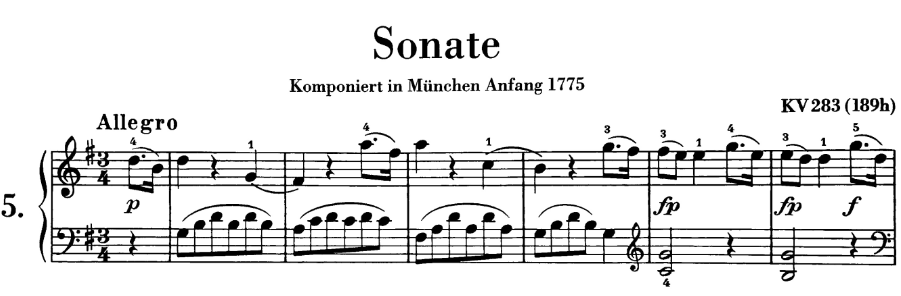
\includegraphics{/images/18-mozart-snippet.png}
\end{figure}
\begin{figure}
  \marginnote{mn-scheme}{
    Symbolic differentiation in Scheme (\href{https://mitp-content-server.mit.edu/books/content/sectbyfn/books_pres_0/6515/sicp.zip/full-text/book/book-Z-H-16.html#%25_sec_2.3.2}{example 2.3.2} in \href{https://en.wikipedia.org/wiki/Structure_and_Interpretation_of_Computer_Programs}{SICP}).
  }
  \begin{code}[scheme]
(define (deriv exp var)
  (cond ((number? exp) 0)
        ((variable? exp)
         (if (same-variable? exp var) 1 0))
        ((sum? exp)
         (make-sum (deriv (addend exp) var)
                   (deriv (augend exp) var)))
        ((product? exp)
         (make-sum
           (make-product (multiplier exp)
                         (deriv (multiplicand exp) var))
           (make-product (deriv (multiplier exp) var)
                         (multiplicand exp))))
        (else
         (error "unknown expression type -- DERIV" exp))))
\end{code}
\end{figure}
\subsection{mozart-scheme-resources}{Resources}

If you want to learn more about Mozart:
\begin{itemize}
    \item
    Listen to the \href{https://www.thegreatcourses.com/courses/great-masters-mozart-his-life-and-music}{Great Masters: Mozart---His Life and Music} course by professor \href{https://robertgreenbergmusic.com/}{Robert Greenberg}.
    \item
    Read \href{https://www.amazon.com/Mozart-Life-Maynard-Solomon/dp/0060883448}{Mozart: A Life} by Maynard Solomon.
\end{itemize}

If you want to learn more about Scheme:
\begin{itemize}
    \item
    Read \href{https://mitpress.mit.edu/9780262510875/structure-and-interpretation-of-computer-programs/}{The Structure and Interpretation of Computer Programs} by Harold Abelson and Gerald Jay Sussman.
    It's worth reading even if you don't care about Scheme.
    \item
    Read \href{https://www.amazon.com/Little-Schemer-Daniel-P-Friedman/dp/0262560992/}{The Little Schemer} and related books: \href{https://www.amazon.com/Reasoned-Schemer-MIT-Press/dp/0262535513/}{The Reasoned Schemer}, \href{https://www.amazon.com/Little-Typer-MIT-Press/dp/0262536439/}{The Little Typer}, \href{https://www.amazon.com/Little-Prover-MIT-Press/dp/0262527952/}{The Little Prover}, and \href{https://www.amazon.com/Little-Learner-Straight-Line-Learning/dp/026254637X/}{The Little Learner}.
\end{itemize}

\section{beethoven}{Ludwig van Beethoven}

\href{https://en.wikipedia.org/wiki/Ludwig_van_Beethoven}{Beethoven} is the most influential composer in history.
He single-handedly changed the direction of western music and the role of an artist in society.

One of the few languages worthy of Beethoven would be \href{https://www.haskell.org/}{Haskell}:
\begin{itemize}
  \item
  Beethoven often constructed his music from the interaction and development of small motifs and rhythms, many of which initially seem trivial.
  The art of writing good Haskell code is composing programs from small functions, many of which do not do much when considered in isolation (\href{https://hackage.haskell.org/package/base-4.18.0.0/docs/Prelude.html#v:id}{\code{id}} and \href{https://hackage.haskell.org/package/base-4.18.0.0/docs/Data-Function.html#v:fix}{\code{fix}}, for example).
  \item
  Beethoven was constantly evolving his style, pushing the boundary of musical art.
  He reinvented himself three times during his career, turning his suffering into fuel for a breakthrough.
  Similarly, the Haskell ecosystem constantly evolves, turning pain points into new beautiful ways to write and think about software.
  For example, issues with lazy input/output led to the invention of \href{https://wiki.haskell.org/Iteratee_I/O}{iteratees}, and problems with nested record updates led to optics (such as \href{https://www.youtube.com/watch?v=k-QwBL9Dia0}{lenses}) and \href{https://www.cis.upenn.edu/~bcpierce/papers/icmt-2009-slides.pdf}{bidirectional programming}.
  \item
  Beethoven turned my musical world upside down: I caught a piano bug after hearing one of his sonatas.
  Haskell enormously influenced my professional life, forever changing my thoughts about computing.
\end{itemize}

\begin{figure}[grayscale-diagram]
  \marginnote{mn-repr-beethoven}{
    Representative Beethoven's music: \href{https://www.youtube.com/watch?v=SrcOcKYQX3c&t=7s}{Sonata op. 13 in C minor}, also known as the Pathétique Sonata.
    Note the operatic dramatism, the masterful use of piano's sonority, and Beethoven's way of building music landscapes from tiny memorable motifs and rhythms.
  }
  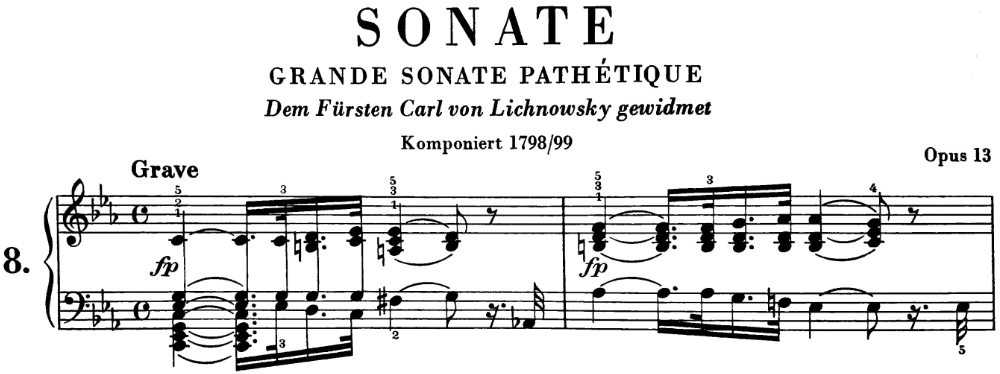
\includegraphics{/images/18-beethoven-snippet.png}
\end{figure}

\begin{figure}
  \marginnote{mn-haskell-example}{
    An idiomatic implementation of the \href{https://en.wikipedia.org/wiki/Knuth%E2%80%93Morris%E2%80%93Pratt_algorithm}{Knuth-Morris-Pratt} algorithm in Haskell.
    The code comes from the \href{https://www.twanvl.nl/blog/haskell/Knuth-Morris-Pratt-in-Haskell}{Knuth-Morris-Pratt in Haskell} article by Twan van Laarhoven.
  }
  \begin{code}[haskell]
data KMP a = KMP { done :: Bool, next :: (a -> KMP a) }

makeTable :: Eq a => [a] -> KMP a
makeTable xs = table
   where table = makeTable' xs (const table)

makeTable' []     failure = KMP True failure
makeTable' (x:xs) failure = KMP False test
   where  test  c = if c == x then success else failure c
          success = makeTable' xs (next (failure x))

isSublistOf :: Eq a => [a] -> [a] -> Bool
isSublistOf as bs = match (makeTable as) bs
   where  match table []     = done table
          match table (b:bs) = done table || match (next table b) bs
\end{code}
\end{figure}

\subsection{beethoven-haskell-resources}{Resources}

If you want to learn more about Beethoven:
\begin{itemize}
  \item
  Listen to the \href{https://www.thegreatcourses.com/courses/great-masters-beethoven-his-life-and-music}{Great Masters: Beethoven---His Life and Music} course by professor \href{https://robertgreenbergmusic.com/}{Robert Greenberg}.
  \item
  Read \href{https://www.amazon.com/Beethoven-Revised-Maynard-Solomon/dp/0825672686}{Beethoven} by Maynard Solomon.
  \item
  Consider watching the \href{https://www.imdb.com/video/vi2964193561/}{Immortal Beloved} movie.
  The movie has many factual mistakes, but it's inspiring nevertheless.
\end{itemize}

If you want to learn more about Haskell:
\begin{itemize}
  \item
  Read \href{http://www.learnyouahaskell.com/}{Learn You a Haskell for Great Good!} by Miran Lipovača.
  It's an engaging and illustrated introduction to Haskell.
  \item
  Read \href{https://www.euterpea.com/haskell-school-of-music/}{The Haskell School of Music} by Paul Hudak and Donya Quick.
  The authors show the best sides of Haskell when they apply it to building a library for music generation.
  \item
  Check out the \href{https://www.haskell.org/documentation/}{Haskell Documentation} page for more great pointers.
\end{itemize}

\section{scriabin}{Alexander Nikolayevich Scriabin}

\href{https://en.wikipedia.org/wiki/Alexander_Scriabin}{Scriabin} is a relatively obscure (at least outside of Russia) Russian composer.
I find his music deeply expressive, emotional, and metaphysical.
Also, he had the most stylish mustache ever.

Scriabin would love \href{https://scala-lang.org/}{Scala}:
\begin{itemize}
  \item
  Scriabin dreamed of fusing arts into a synthetic art form he called \href{https://en.wikipedia.org/wiki/Mysterium_(Scriabin)}{Mysterium}.
  Similarly, Scala aims to be extensible enough to embrace all programming styles and paradigms (functional, object-oriented, actor-based, etc.).
  \item
  Scriabin's music feels profound and unfathomable, like the night sky.
  Looking at Scala code makes me feel the same awe: I admire its structure and elegance, but its inherent complexity makes my head spin.
\end{itemize}

\begin{figure}[grayscale-diagram]
  \marginnote{mn-repr-scriabin}{
    Representative Scriabin's music: \href{https://www.youtube.com/watch?v=Uy8MTTrh-Z8&t=709s}{Prelude in C#-minor from op. 11}, one of my favorite short piano pieces.
  }
  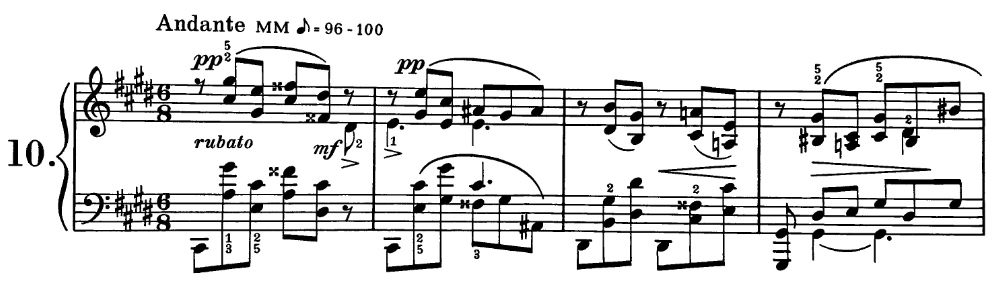
\includegraphics{/images/18-scriabin-snippet.png}
\end{figure}
\begin{figure}
\marginnote{mn-scala-snippet}{
  The Scala way of saying that optional values are just an instance of a monoid in the category of endofunctors.
  This snippet comes from the \href{https://github.com/scalaz/scalaz#type-class-instance-definition}{\code{scalaz}} library documentation.
}
\begin{code}[scala]
implicit val option: Traverse[Option] with MonadPlus[Option] =
  new Traverse[Option] with MonadPlus[Option] {
    def point[A](a: => A) = Some(a)
    def bind[A, B](fa: Option[A])(f: A => Option[B]): Option[B] = fa flatMap f
    override def map[A, B](fa: Option[A])(f: A => B): Option[B] = fa map f
    def traverseImpl[F[_], A, B](fa: Option[A])(f: A => F[B])(implicit F: Applicative[F]) =
      fa map (a => F.map(f(a))(Some(_): Option[B])) getOrElse F.point(None)
    def empty[A]: Option[A] = None
    def plus[A](a: Option[A], b: => Option[A]) = a orElse b
    def foldR[A, B](fa: Option[A], z: B)(f: (A) => (=> B) => B): B = fa match {
      case Some(a) => f(a)(z)
      case None => z
    }
}
\end{code}
\end{figure}

\subsection{scriabin-cl-resources}{Resources}

If you want to learn more about Scriabin:
\begin{itemize}
  \item
  Read \href{https://www.amazon.com/Alexander-Scriabin-Companion-History-Performance/dp/1442232617/}{The Alexander Scriabin Companion: History, Performance, and Lore} by Lincoln Ballard and Matthew Bengtson.
  \item
  Read \href{https://www.amazon.com/Scriabin-Biography-Second-Revised-Dover/dp/0486288978/}{Scriabin, a Biography} by Faubion Bowers.
\end{itemize}

If you want to learn more about Scala:
\begin{itemize}
    \item
    Read \href{https://www.amazon.com/Programming-Scala-Fifth-Odersky-dp-0997148004/dp/0997148004/}{Programming in Scala} by Martin Odersky et al., and \href{https://www.amazon.com/gp/product/1617290653/}{Functional Programming in Scala} by Rúnar Bjarnason and Paul Chiusano.
\end{itemize}

\section{closing}{Closing words}

There are many more great composers and excellent programming languages.
Matching these is an exercise for the reader.

I encourage you to think more often about things and people you like and match them with others.
For example, \href{https://kpknudson.com/my-favorite-theorem/}{My Favorite Theorem} podcast hosts ask their guests to match their favorite theorems with items and activities in their lives, such as pizza and rock climbing.

Enjoy your \href{https://www.youtube.com/watch?v=2G6dd7ikrXs}{favorite things}!
\end{document}
